% Print results for comparing MSN with Heaviside jump function

\begin{figure}[p]
    \centering
    \begin{subfigure}{0.45\textwidth}
    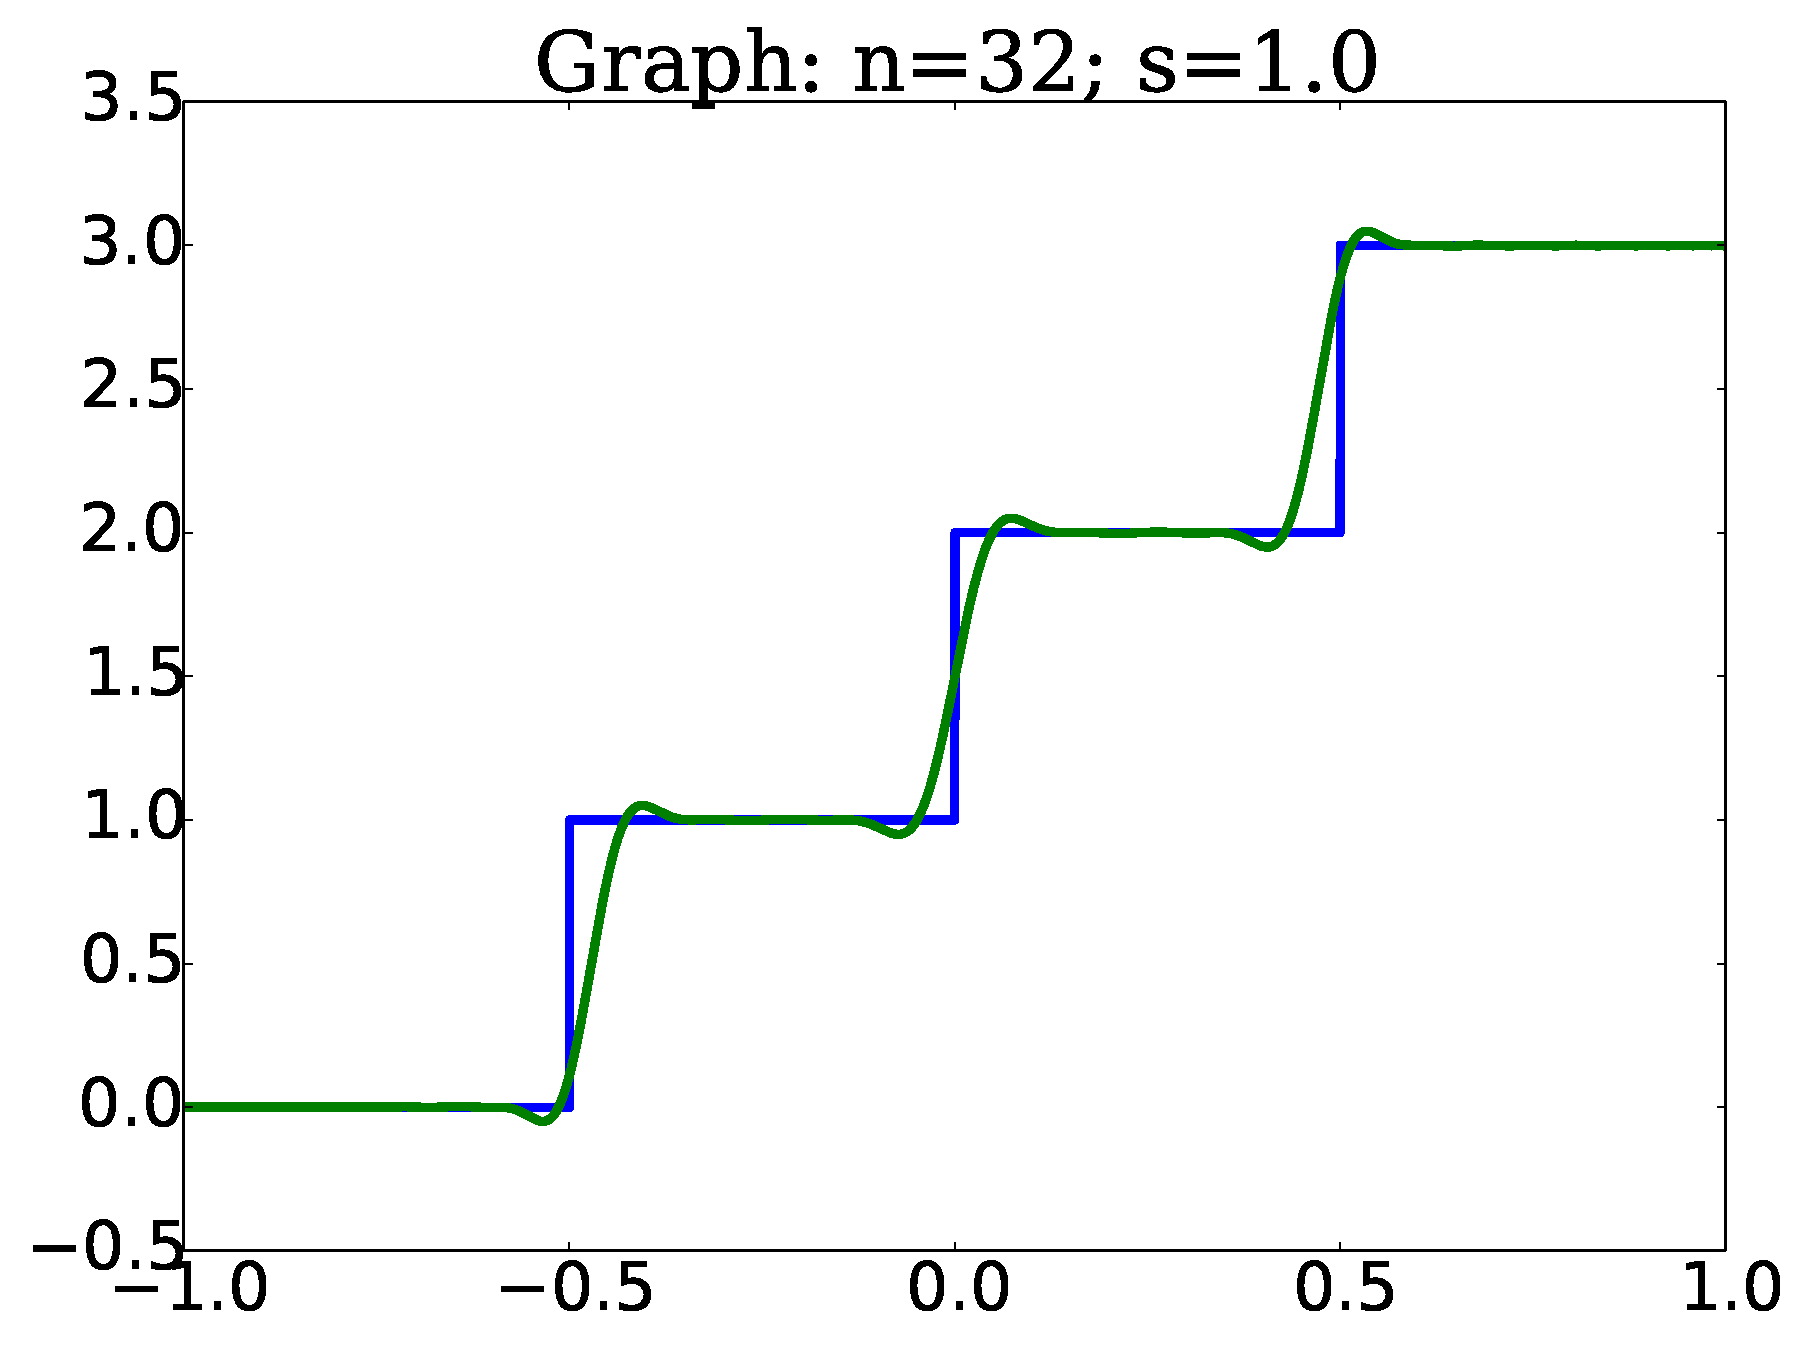
\includegraphics[width=\textwidth]{plots/graph_n_32_s_1_heaviside_2.pdf}
    \end{subfigure}
    \begin{subfigure}{0.45\textwidth}
    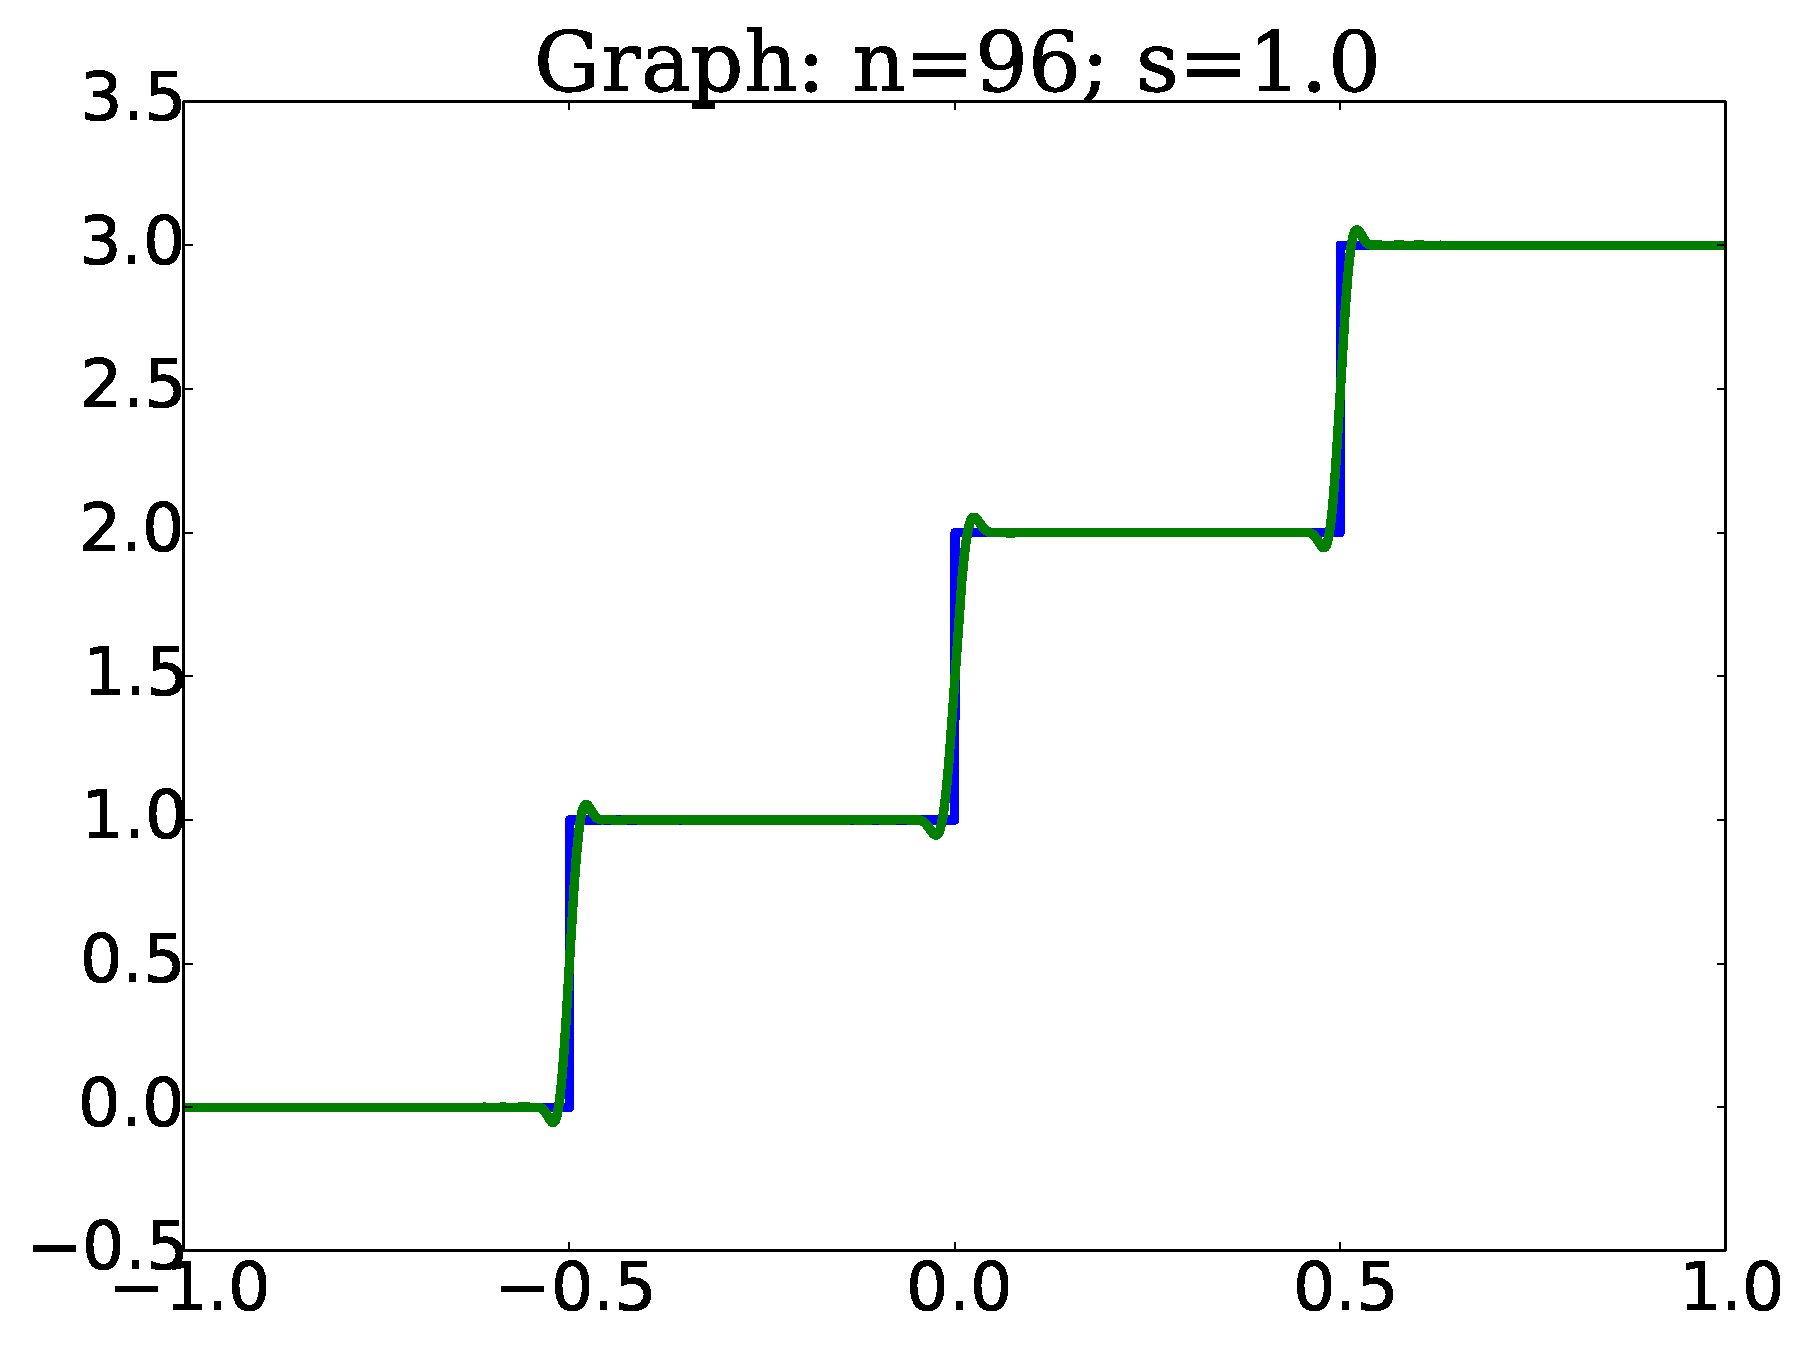
\includegraphics[width=\textwidth]{plots/graph_n_96_s_1_heaviside_2.pdf}
    \end{subfigure}

    \begin{subfigure}{0.45\textwidth}
    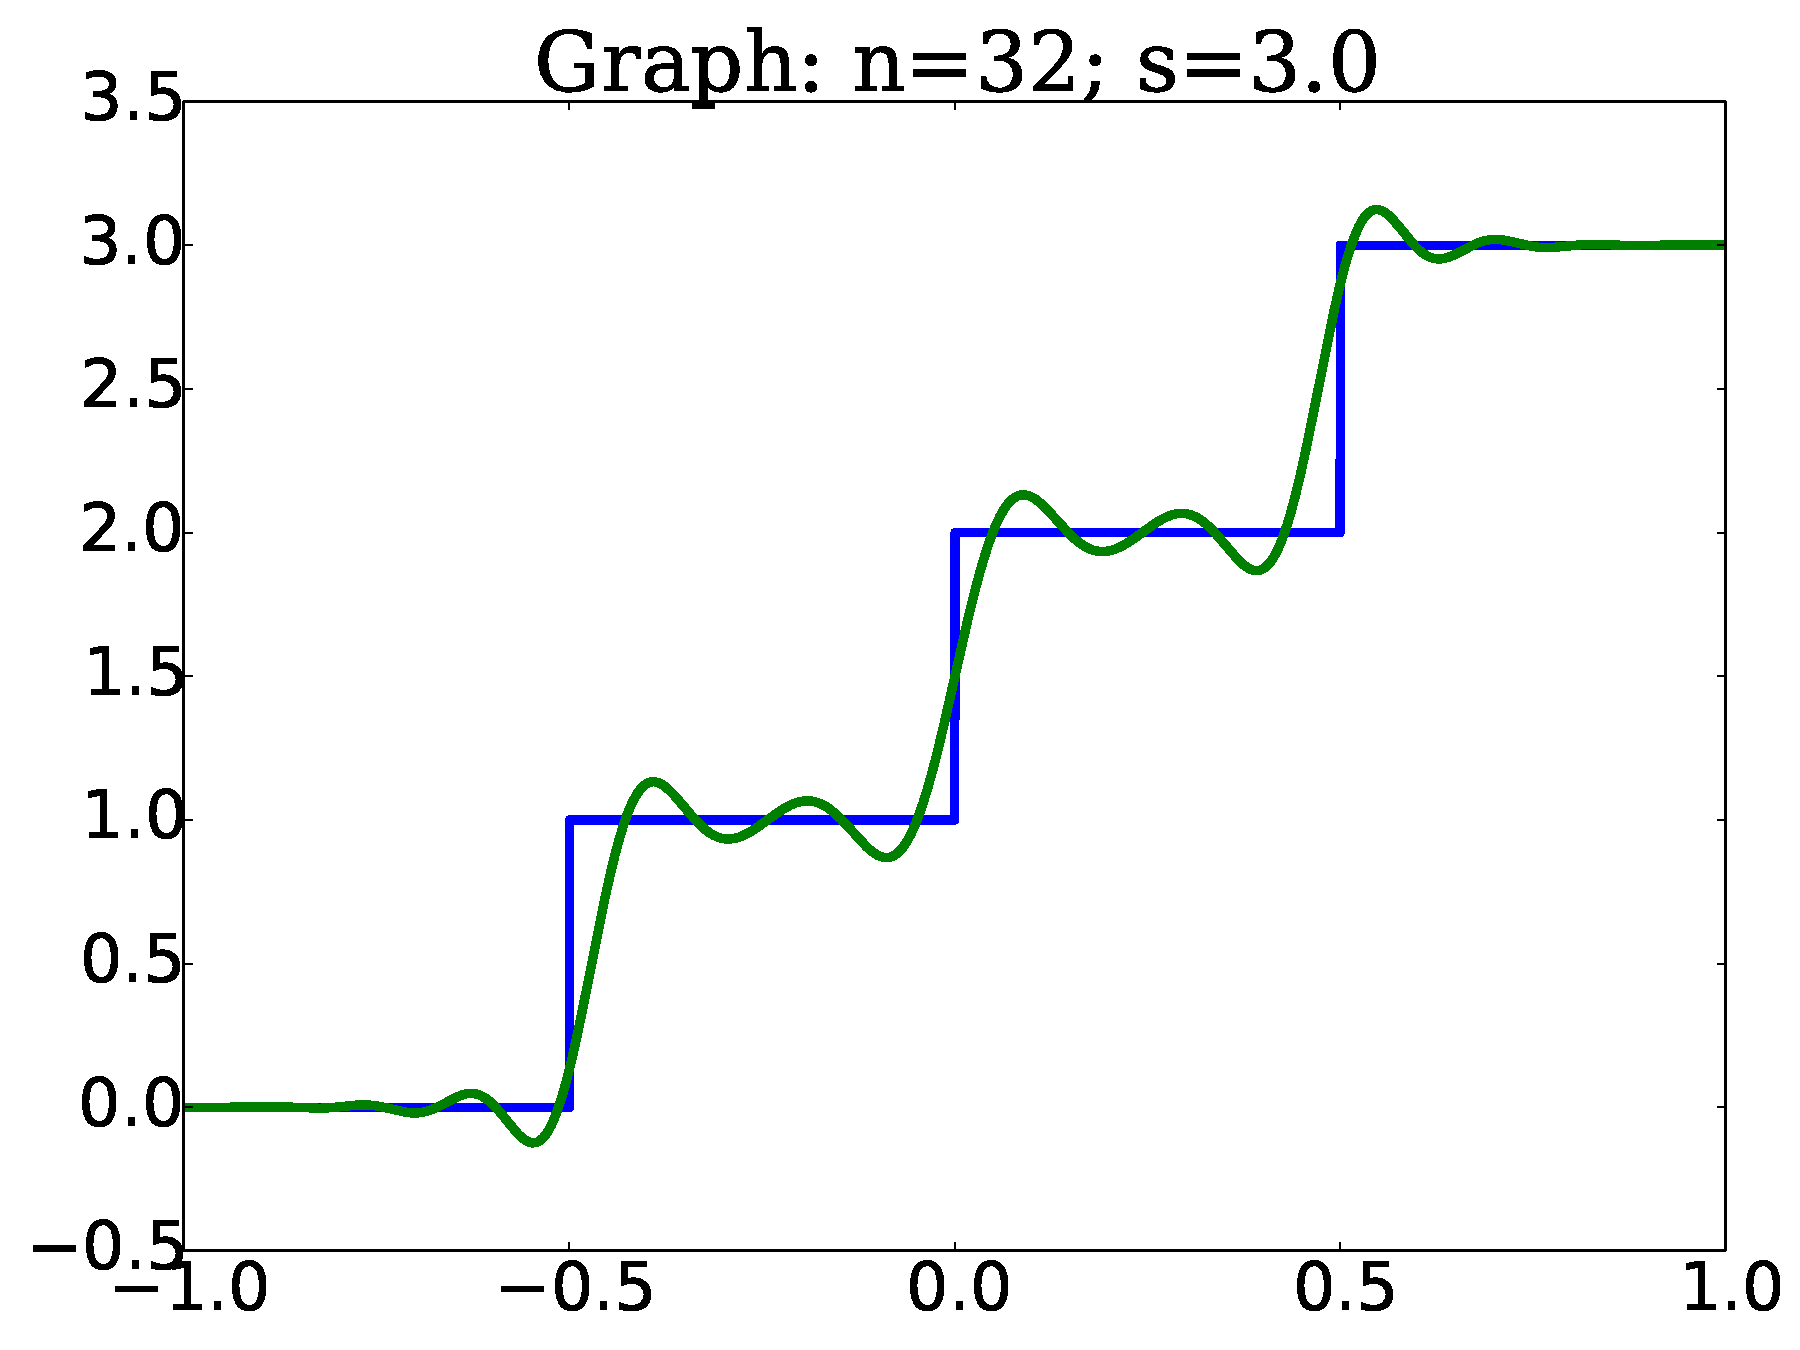
\includegraphics[width=\textwidth]{plots/graph_n_32_s_3_heaviside_2.pdf}
    \end{subfigure}
    \begin{subfigure}{0.45\textwidth}
    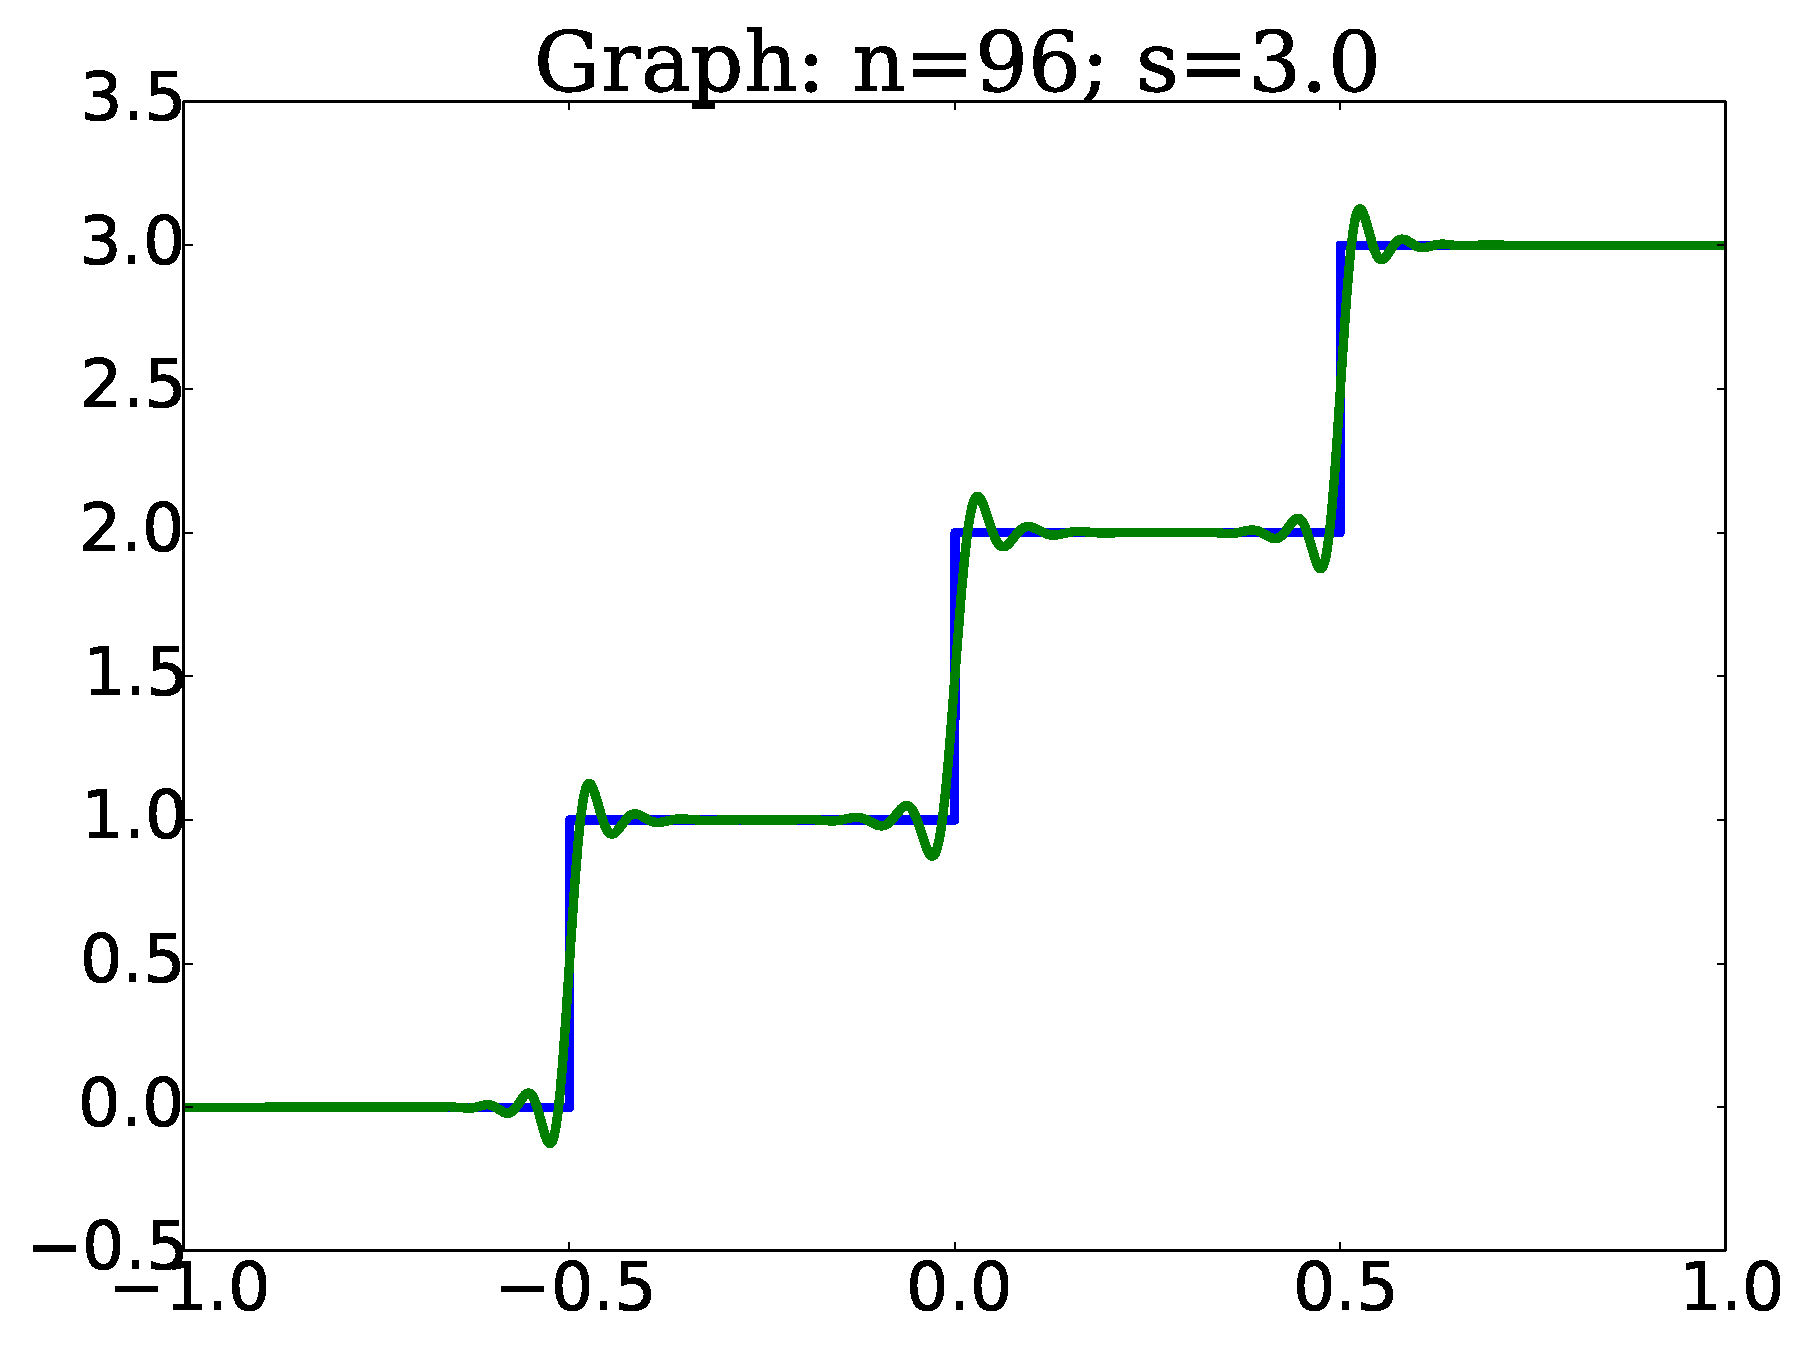
\includegraphics[width=\textwidth]{plots/graph_n_96_s_3_heaviside_2.pdf}
    \end{subfigure}

    \begin{subfigure}{0.45\textwidth}
    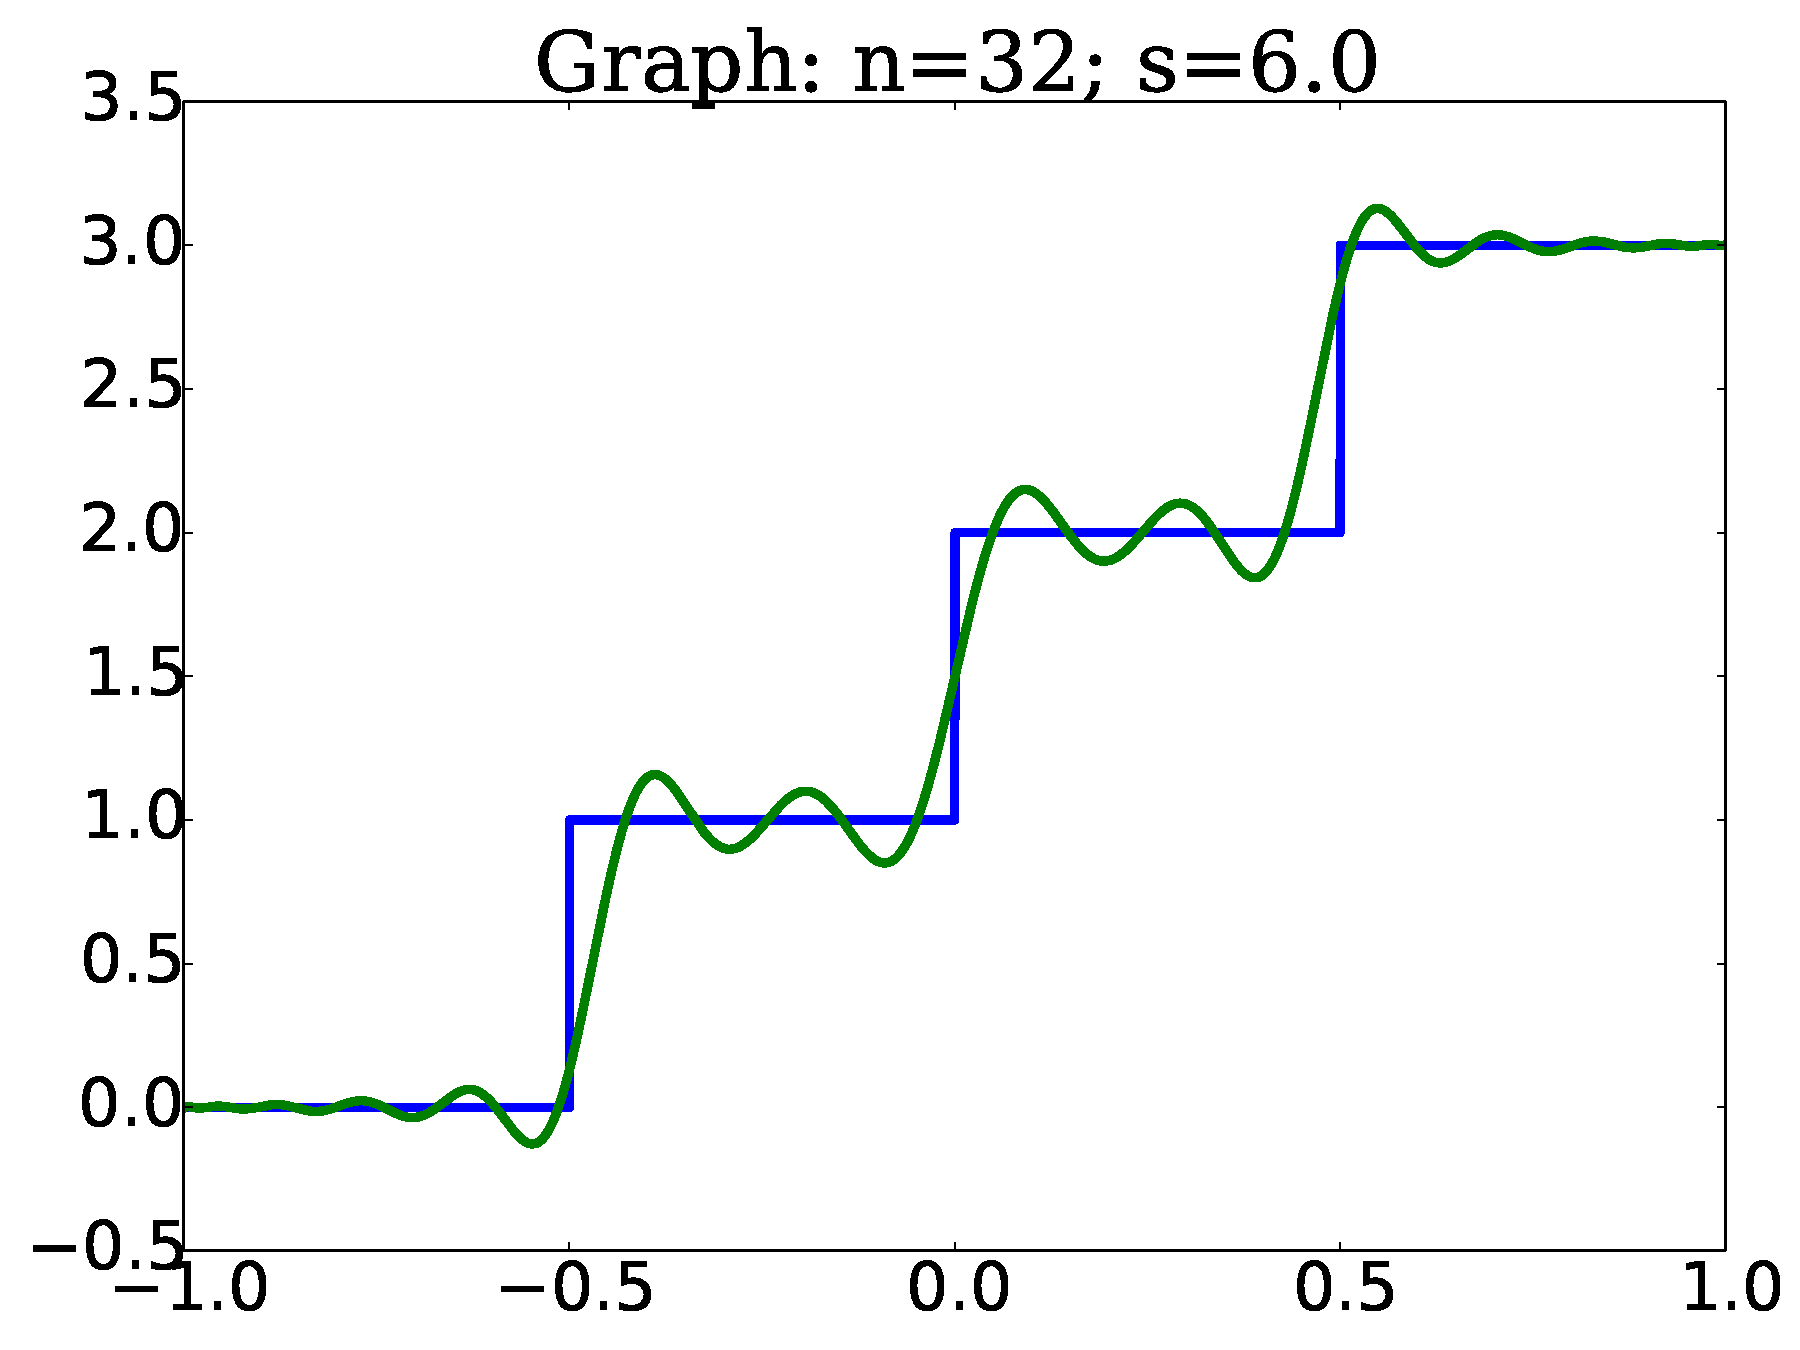
\includegraphics[width=\textwidth]{plots/graph_n_32_s_6_heaviside_2.pdf}
    \end{subfigure}
    \begin{subfigure}{0.45\textwidth}
    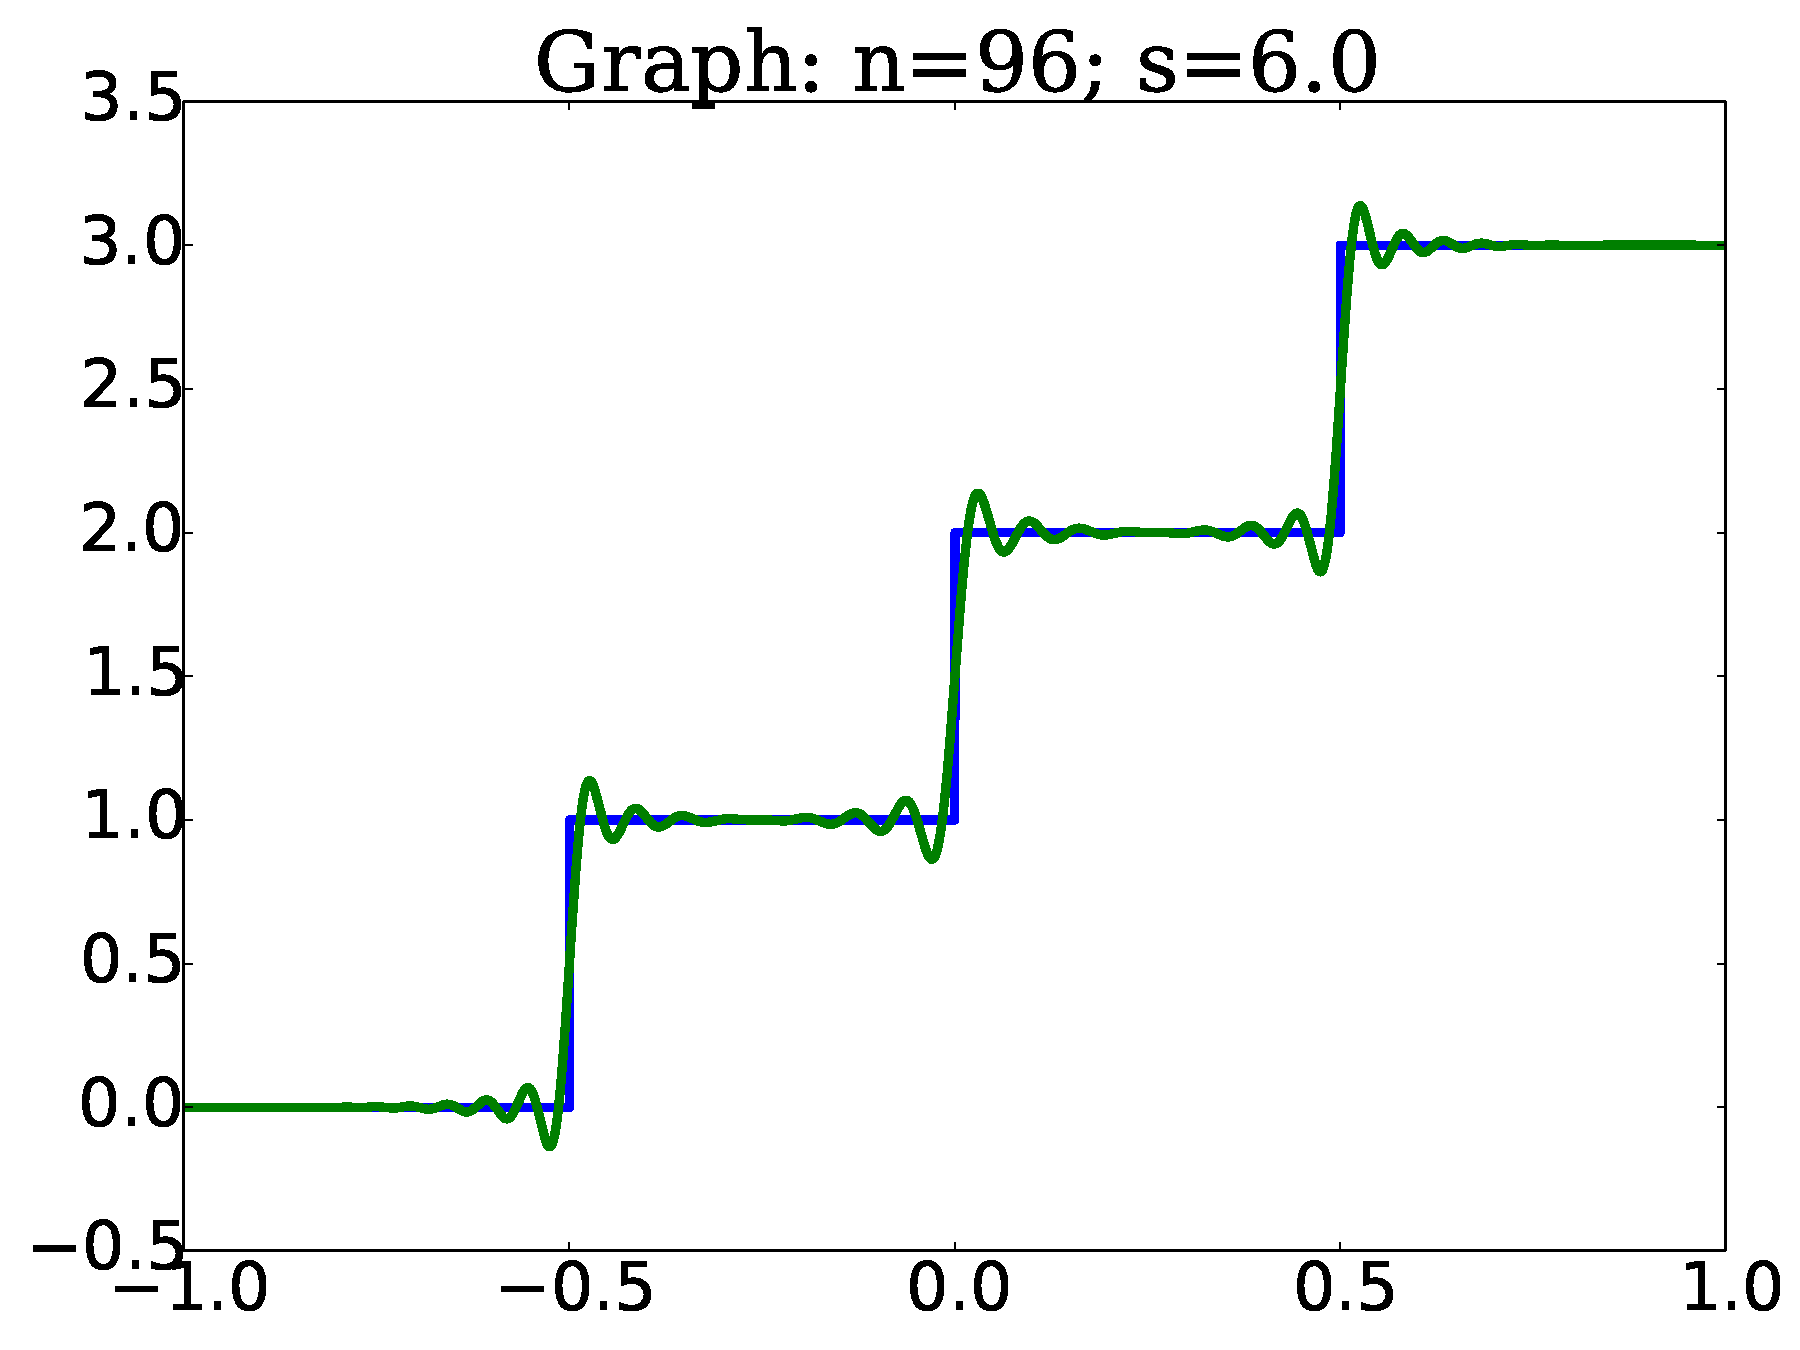
\includegraphics[width=\textwidth]{plots/graph_n_96_s_6_heaviside_2.pdf}
    \end{subfigure}
\caption[Example Plots of MSN Interpolation of Rough Functions]{
We plot MSN approximations against the true solution $H_{2}$
for various $s$ and $n$ values.
}
\label{fig:msn_n_s_heaviside_2}
\end{figure}



